\subsection{Usage Behavior}
\label{subsec:behavior}

To characterize diurnal user behavior as observed at the ISP, we first calculate
usage per subscriber (table ~\ref{tab:eval-criteria}), and then plot the median and
90\%-ile of total usage over a week for both \test and \control
sets (figure~\ref{fig:TS-data-rate-daily}).

We observe that the rise to the peak prime time hour usage on weekdays
is not plateaued like the pattern observed on weekends (and holidays).
A generic (median) weekday aggregate usage consists of a rise in usage that starts
early in the morning that builds up to the prime-time period, peaks, and then falls sharply.
We do not observe a trough in mid afternoon (between 2:00 PM -- 6:00 PM), as is usually
the case for overall usage observed at US Fixed access providers ~\cite{sandvine2014report1}.

\begin{figure}[ht!]
\begin{minipage}{\linewidth}
  \centering
  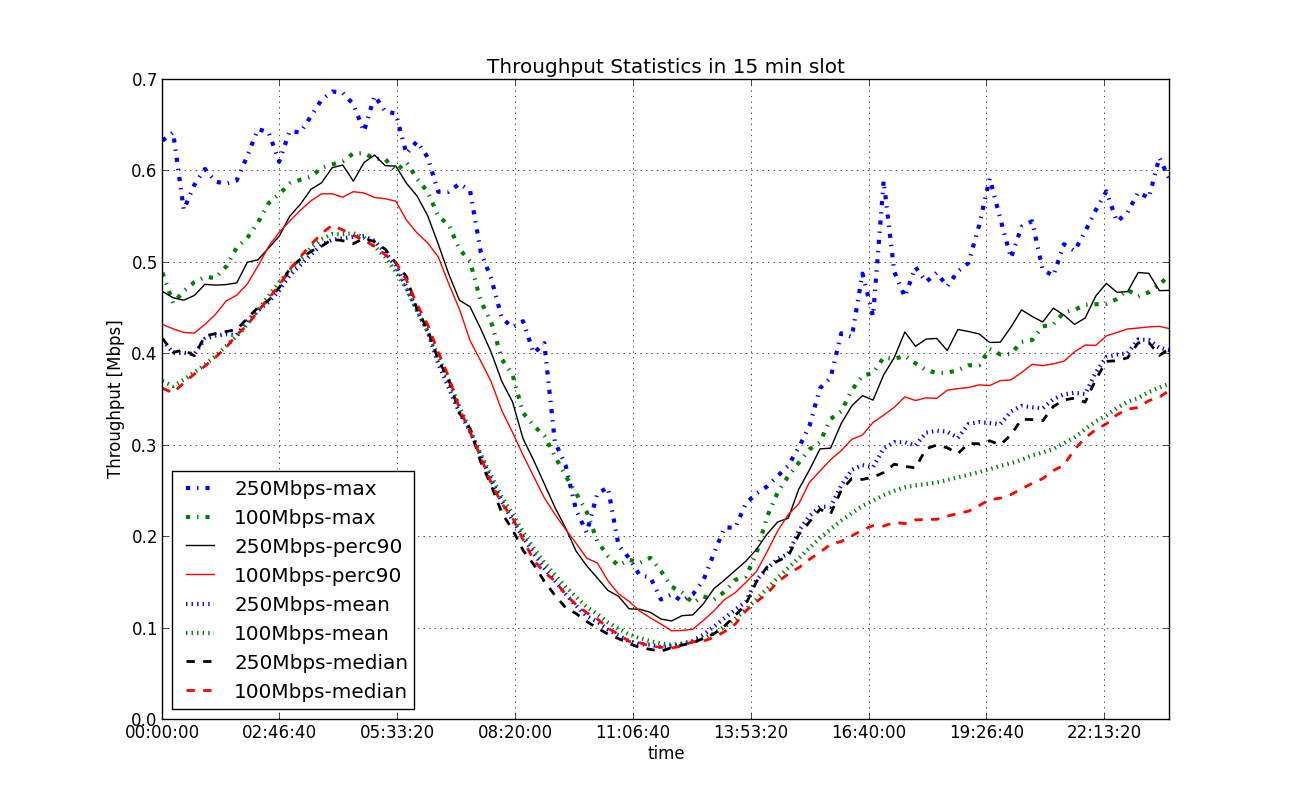
\includegraphics[width=\linewidth]{figures/describe-total-throughput-per-day[replace].png}
  \caption{agg (days) over means (devices): aggregate has no trough, peaks in the evening hours}
  %http://riverside.noise.gatech.edu:8083/separated/full/describe-total-throughput-per-day.png
  \label{fig:TS-data-rate-daily}
\end{minipage}
\end{figure}

Comparing the \test and \control sets, we observe that the median prime time and late night
behavior is very similar (7:00 PM -- 7:00 AM), but during off peak daytime (work) hours,
the \test set has a higher median than the \control set. There was no change in
prime time behavior in the evening, and an increased usage in off-peak daytime hours.

% EXPLAIN:
% LACK OF TROUGHS: users' behavior in higher tier bandwidth
% DISCREPANCY IN DAYTIME OFFPEAK: ??? 

\todo{see todo.txt for analysis comments, things to explain, things to check}